\section{Directed Khepera (class)}
\label{sec:dk}

\subsection{Introduction}
\label{sec:dk:intro}

This class aims to pilot the \khepera{} to a given ($x$, $y$) position. 
To do 
so, we get the position and orientation of the Khepera from a camera 
hanging from the ceiling. It needs to calculate the needed orientation 
to drive to a ($x$, $y$) position and sends a command to the Khepera via a 
serial port to make it turn or drive forward.

\subsection{Communication}
\label{sec:dk:comm}

It first opens a port for serial port communication. The serial port 
communicates via Bluetooth. In Ubuntu, it is usually “/dev/rfcomm0”.

To write commands to the buffer, it is imperative to add a carriage '$\backslash$r' 
at the end. If not, the Khepera will not recognize the command. 

The buffer is read char by char. The robot always answers to commands. 
The buffer is emptied after every command that is sent.

\subsection{Navigation}
\label{sec:dk:nav}

    \marginpar{
        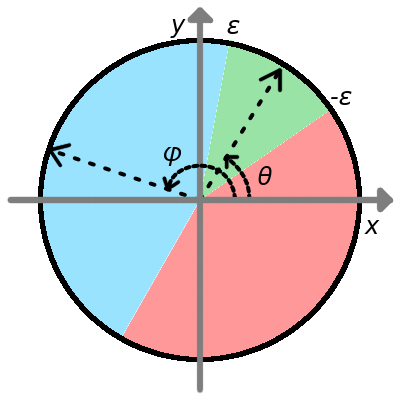
\includegraphics[width=4.5cm]{./img/desiredangle.png}
        \captionof{figure}[Navigation based on desired angle]{%
        Navigation based on desired angle --
        The desired angle $\varphi$ is the orientation needed
        to access the ($x_{target}$, $y_{target}$) position 
        in straight line. $\theta$ is the current orientation
        of the robot. If $\varphi$ falls in the blue region 
        regarding $\theta$, then the robot should turn left. If
        $\varphi$ falls in the green region regarding $\theta$, 
        then the robot should go forward. Finally, if $\varphi$ 
        falls in the red region regarding $\theta$, the robot should
        turn right.}
        \label{fig:dk:nav}
    }
 
    \begin{enumerate}
        \item It first get the position of the robot including 
            the orientation. 
        \item If the detection is not successful and position is unknown, 
            it sends a command to immobilize the robot
        \item It then calculates the desired angle 
            $ \varphi = $
            atan2($y_{t}-y_{target}$, $x_{t}-x_{target}$)
        \item It add $\pi$ to the calculated angle and the robot orientation 
            to get range (0, 2$\pi$) rather than ($-\pi$, $\pi$)
        \item Angle error $\alpha = \varphi-\theta$ 
        \item If $|\alpha| < \epsilon_\theta$ (if $\varphi$ fall in green 
            region in figure 
            \ref{fig:dk:nav})
            it sends a forward command
        \item If $\epsilon_\theta < |\alpha| < \pi$ (if $\varphi$ fall in
            red region in figure \ref{fig:dk:nav})
            sends a turn right command
        \item Else ($\varphi$ fall in blue region in figure \ref{fig:dk:nav}) 
              sends a turn left command
        \item Do this while $(x_t-x_{target})^2+(y_t-y_{target})^2 > \epsilon_e^2$ 
    \end{enumerate}

$\epsilon_\theta$ and $\epsilon_e$ are statically defined in the class.

The turn right and turn left commands are graded on the level of angle 
error. To simplify calculations, negative angle errors,
are inverted by adding 
2$\pi$ before calculating turning speed. The function of the speed, $sp$, 
is the following, where $sp_{min}$ and $sp_{max}$ are respectively the
minimal and maximal speed of the robot:

\begin{displaymath}
    Sp = \left(\frac{1}{\pi-\epsilon_\theta}\right)\left(\alpha*(sp_{max}-sp_{min}) + 
\pi*sp_{min}-\epsilon_\theta*sp_{max}\right)
\end{displaymath}

\subsection{Improvements}
\label{sec:dk:improvements}

There is no command for the robot for a definite angle rotation. It 
would be a great enhancement for the rapidity and accuracy of the robot 
movements if we could find a way to make it precise turns of a given 
angle with a single command. There is a command to make precise turn 
of the wheels, but it doesn’t interpolate directly to a complete robot 
rotation of a precise angle. We would need to calculate how much the 
Khepera moves for a precise rotation of the wheels.
\\
\\
The update of the tapir detector and the time between read/write commands 
on the buffer of the serial port are really slow. The tapir detector 
seems to update values at a rate between 1 to 2 times per second, 
which is incredibly slow. It would be really helpful to speed up both 
processes to get higher accuracy in the navigation.

\subsection{How to use}
\label{sec:dk:howto}
The tapir detector must be on. Set parameters of the tapir detector in 
khepera\_tapir.cfg. To learn how to set up the Bluetooth connection, 
take a look at the section \ref{sec:howto:khepera}.

\subsubsection{Constructor parameters}
\label{sec:dk:howto:constparams}
    \begin{description} \itemindent=-15pt
        \item[PORT] port of the serialport. Usually “/dev/rfcomm0” in 
            Ubuntu.
        \item[max\_speed, min\_speed (optional)] Be carefull if you set 
            those parameters. The update time of the detector is slow 
            and serial port communication too, so if the max\_speed is 
            too high, there might be overruns.
    \end{description}

\subsubsection{Init parameters}
\label{sec:dk:howto:initparams}
    \begin{description} \itemindent=-15pt
        \item[manipulate] If true, the robot enters an infinite loop where 
            you can send commands. Write “quit” to end, it then returns 
            false and CLsquare ends.
        \item[delta\_t] The sleep time between each loop of the 
            navigation algorithm. Delta\_t seems to need to be equal 
            or higher than 1.0 second because of the time that 
            takes Tapir.update() and write/read serial port commands.
    \end{description}
